% radar_tradeoffs_full.tex -- self-contained standalone radar plot figure
\documentclass[tikz]{standalone}
\usepackage{pgfplots}
\pgfplotsset{compat=1.18}
\usepackage{siunitx}

\begin{document}
\begin{figure}[h!]
\centering
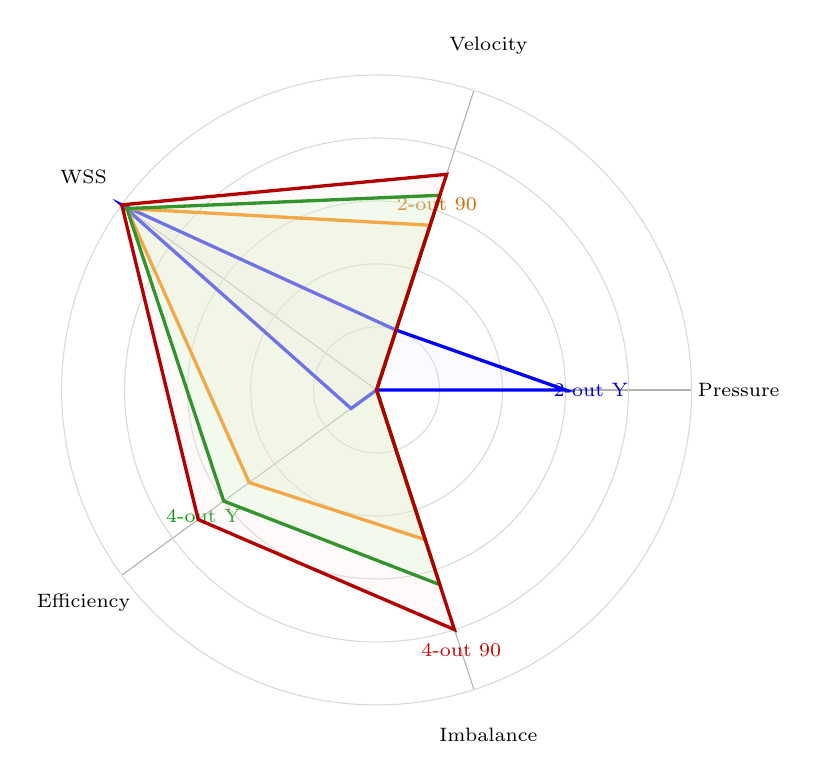
\begin{tikzpicture}[scale=4]

% Define the categories
\def\categories{5}
\def\labels{{"Pressure", "Velocity", "WSS", "Efficiency", "Imbalance"}}

% Draw radial lines and labels
\foreach \i in {1,...,\categories} {
  \pgfmathsetmacro\angle{(360/\categories)*(\i-1)}
  \draw[gray!60] (0,0) -- (\angle:1);
  \node[font=\scriptsize] at (\angle:1.15) {\pgfmathparse{\labels[\i-1]}\pgfmathresult};
}

% Draw concentric rings
\foreach \r in {0.2,0.4,0.6,0.8,1.0} {
  \draw[gray!30] (0,0) circle (\r);
}

% --- DATA: normalized (0-1) ---

% 2-out Y (drawn last to avoid hiding others)
\draw[very thick, draw=blue, fill=blue!10, fill opacity=0.2] plot coordinates {
  (0:0.6)
  (72:0.2)
  (144:1.0)
  (216:0.1)
  (288:0.0)
} -- cycle;
\node[blue!80!black, font=\scriptsize] at (0:0.68) {2-out Y};

% 2-out 90
\draw[very thick, draw=orange, fill=orange!20, fill opacity=0.2] plot coordinates {
  (0:0.0)
  (72:0.55)
  (144:0.98)
  (216:0.5)
  (288:0.5)
} -- cycle;
\node[orange!80!black, font=\scriptsize] at (72:0.62) {2-out 90};

% 4-out Y
\draw[very thick, draw=green!50!black, fill=green!30, fill opacity=0.2] plot coordinates {
  (0:0.0)
  (72:0.65)
  (144:0.98)
  (216:0.6)
  (288:0.65)
} -- cycle;
\node[green!60!black, font=\scriptsize] at (216:0.68) {4-out Y};

% 4-out 90
\draw[very thick, draw=red!70!black, fill=red!10, fill opacity=0.2] plot coordinates {
  (0:0.0)
  (72:0.72)
  (144:1.0)
  (216:0.7)
  (288:0.8)
} -- cycle;
\node[red!80!black, font=\scriptsize] at (288:0.87) {4-out 90};

\end{tikzpicture}
\caption{Radar plot comparing normalized values across five performance dimensions for 2- and 4-outlet Y-split and 90-degree configurations using Alginate 8\% at 105 mBar.}
\label{fig:radar_tradeoffs}
\end{figure}
\end{document}
